% \begin{figure}
%     \centering
%     \begin{subfigure}[b]{0.485\linewidth}
%         \centering
%         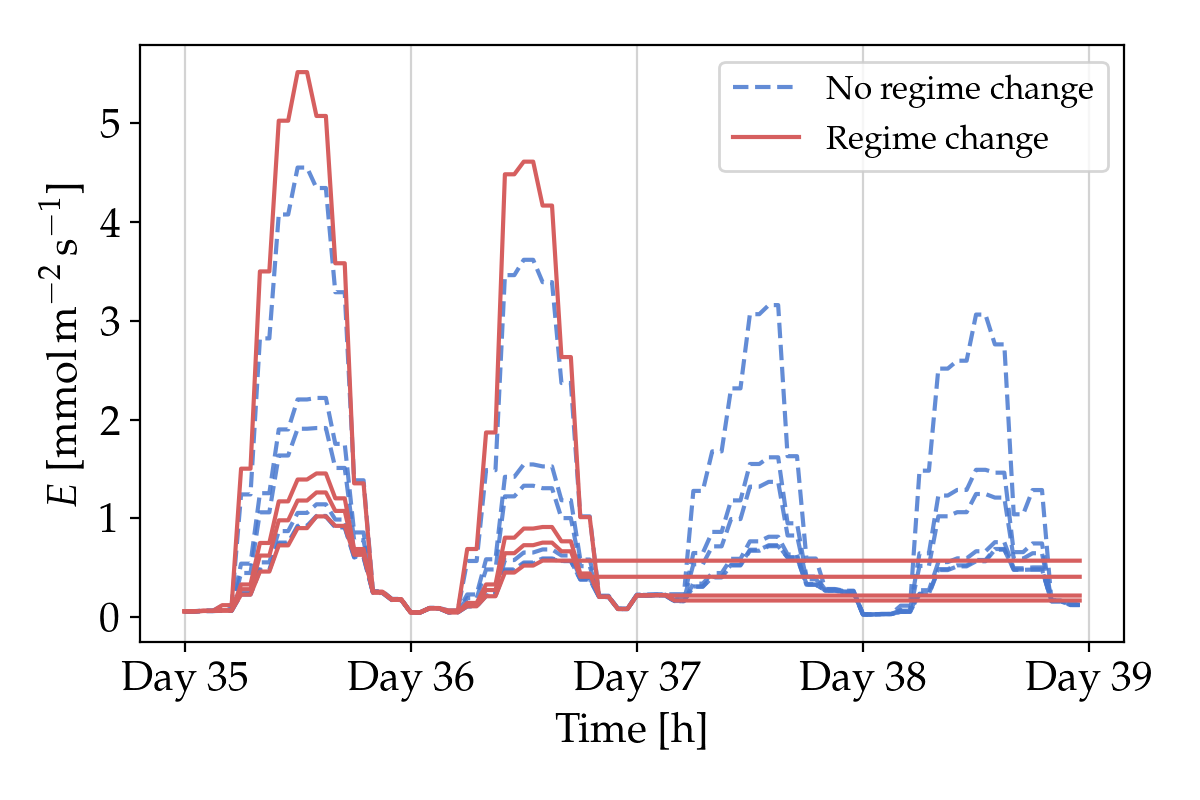
\includegraphics[width=\linewidth,height=\linewidth,keepaspectratio]{img/cn_regime_change.png}
%         \caption{HydroShoot}
%         \label{fig:hydroshoot-archi}
%     \end{subfigure}
%     \hfill
%     \begin{subfigure}[b]{0.485\linewidth}
%         \centering
%         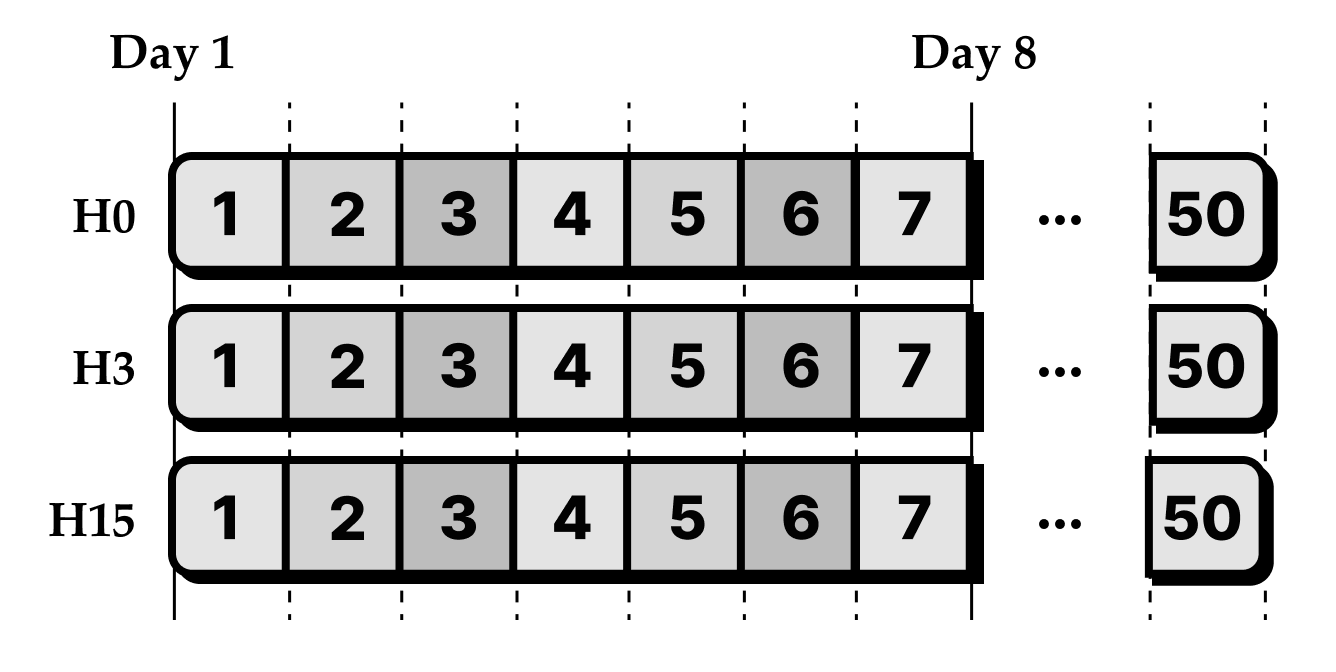
\includegraphics[width=\linewidth,height=0.85\linewidth,keepaspectratio]{img/cnw-grouping.png}
%         \caption{CN-Wheat}
%         \label{fig:cnwheat-archi}
%     \end{subfigure}
%     \caption{
%             FSPMs selected for use in experiments in this work. 
%             (\subref{fig:hydroshoot-archi}) A grapevine specimen from HydroShoot with the canopy trained in the ``Geneva Double Curtain'' configuration.  This figure is reused from \citet{albasha_hydroshoot_2019} under the CC BY 4.0 license.
%             (\subref{fig:cnwheat-archi}) The architecture of the CN-Wheat model. This figure is reused from \citet{barillot_cn-wheat_2016} with permission from the publisher (Copyright 2016 Oxford University Press).
%     }
%     \label{fig:appendix_cnwheat_figures}
% \end{figure}

\begin{figure}[]
	\centering
    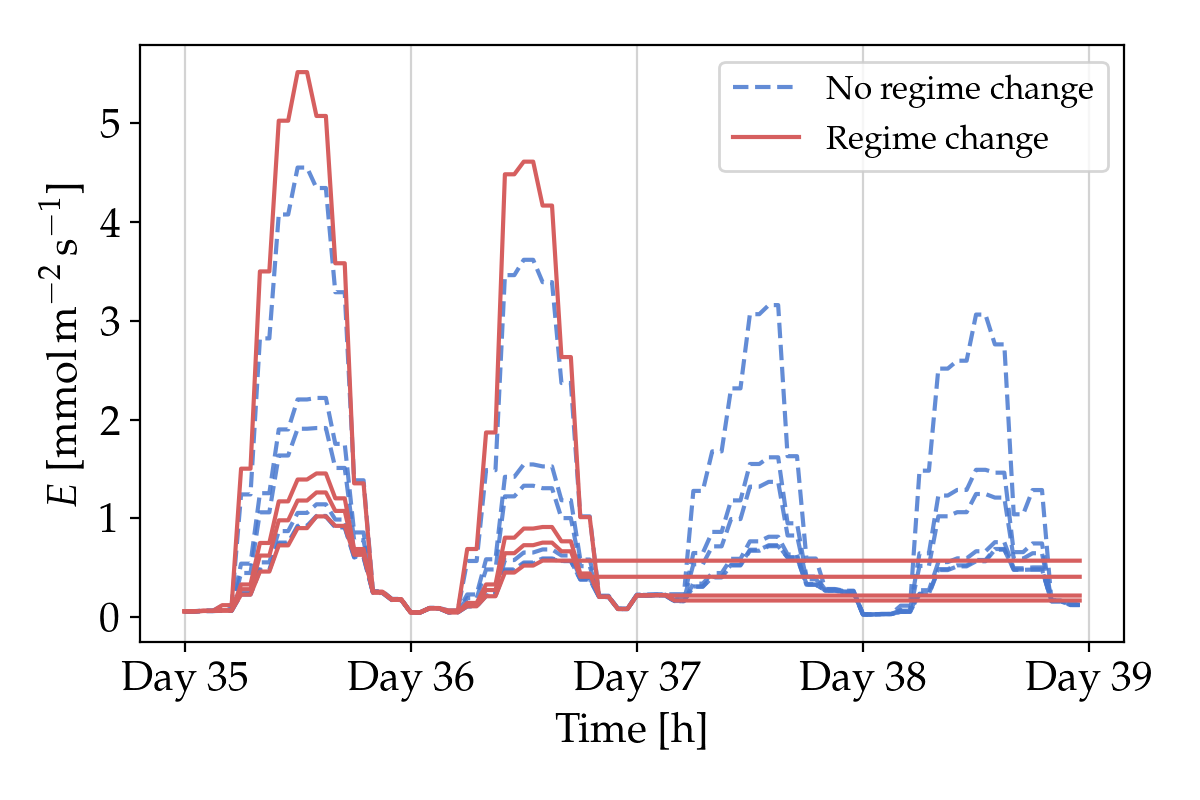
\includegraphics[width=10cm]{img/cn_regime_change.png}
	\caption[Some structural elements of CN-Wheat stop functioning after a specific amount of days.]{Some structural elements of CN-Wheat stop functioning after a specific amount of days. Depicted on the figure is the transpiration rate of each shoot element in the H3 simulation. The red elements change their behavior after day 37.}
	\label{fig:cnwheat-regime-change}
\end{figure}


\begin{figure}[]
	\centering
    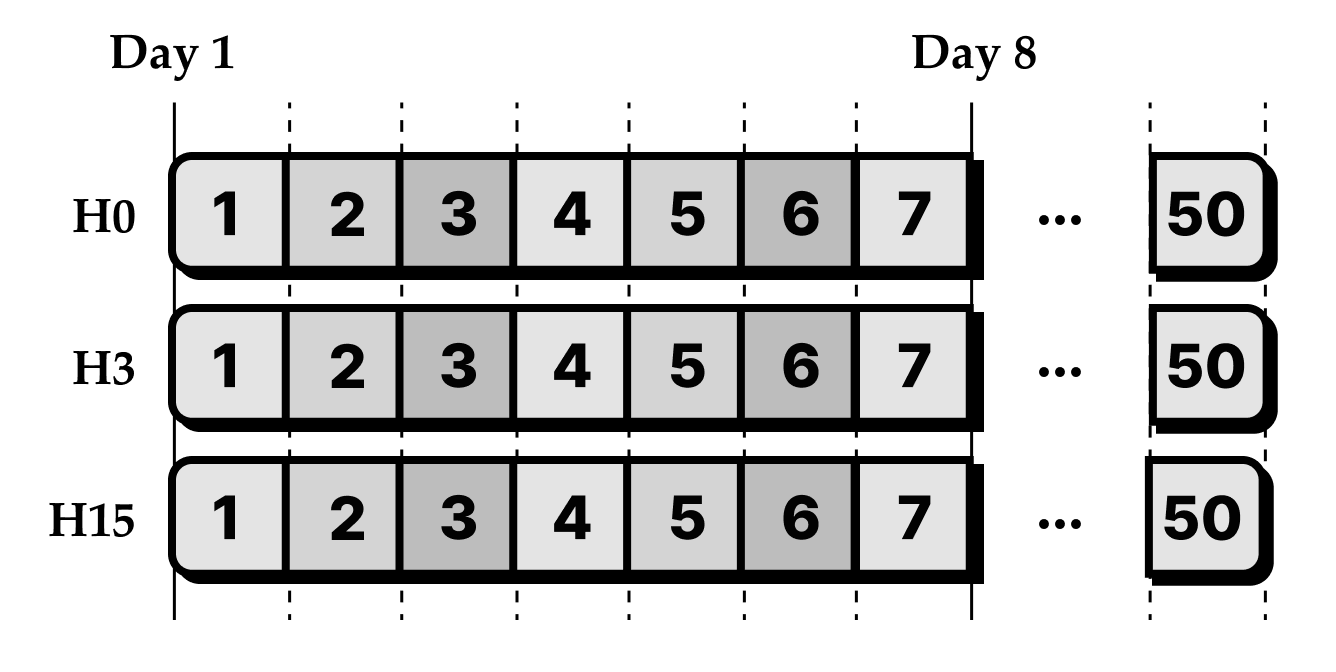
\includegraphics[width=10cm]{img/cnw-grouping.png}
	
	\caption[Data grouping method used to combine data from three simulations of CN-Wheat.]{Data grouping method used to combine data from three simulations of CN-Wheat. Data with the same group number must stay together in a train, validation, or test set.}
	\label{fig:cnwheat-grouping}
\end{figure}